\subsubsection{Sensitivity Analysis}
\label{sec:sensitivity}

The sub-ppm precision of the $\alpha$ prediction depends critically on the backreaction 
coefficient. We analyze the sensitivity to demonstrate this is not fine-tuning but 
a genuine geometric constraint.

\textbf{Exponent variation (diagnostic):}
\begin{center}
\begin{tabular}{@{}ccc@{}}
\toprule
\textbf{Exponent $k$} & $\alpha^{-1}$ & \textbf{Deviation (ppm)}\\
\midrule
$k = 0$ (no backreaction) & 137.03650146 & $+3.67$\\
$k = 1$ & 137.03624686 & $+1.81$\\
$k = 1.5$ & 137.03612025 & $+0.88$\\
$\mathbf{k = 2}$ (double cover) & $\mathbf{\num[round-mode=places,round-precision=10]{\TFPTalphaInvSelfNum}}$ & $\mathbf{-0.037}$\\
$k = 2.5$ & 137.03586841 & $-0.95$\\
$k = 3$ & 137.03574318 & $-1.87$\\
\bottomrule
\end{tabular}
\end{center}

\textbf{Key observations:}
\begin{enumerate}[leftmargin=1.5em, topsep=2pt, itemsep=1pt]
    \item The zero crossing occurs near $k \approx 1.97$ in this diagnostic.
    \item The exponent $k=2$ is not fitted; it follows from the double cover having two sheets.
    \item Sensitivity: $\Delta(\alpha^{-1})/\Delta k \approx 2.5 \times 10^{-4}$ per unit of $k$, 
        or about 1.8 ppm per unit change.
\end{enumerate}

\textbf{Why the exponent must be exactly 2:}

The orientable double cover has exactly two sheets. Field energy on each sheet couples 
identically to the boundary data. Any coefficient $\neq 2$ would require:
\begin{itemize}[leftmargin=1.5em, topsep=2pt, itemsep=1pt]
    \item Asymmetric coupling (violating the cover symmetry), or
    \item Additional sheets (violating the minimal orientable completion), or
    \item A non-geometric origin (abandoning the axiom structure).
\end{itemize}

Although $-0.037$ ppm appears small, CODATA 2022 has $\sigma(\alpha^{-1})\simeq 2.1\times 10^{-8}$, i.e.\ a ppm-scale uncertainty of only $\sim 1.5\times 10^{-4}$ ppm. The one-defect truncation is therefore \emph{excluded} at CODATA precision and is shown here only as a diagnostic baseline; the derived two-defect partition (Sec.~\ref{sec:sensitivity}; Theorem~\ref{thm:selfconsistent}) supplies the required second-order correction.

\TFPTAlphaSensitivityPlot

\begin{figure}[H]
\centering
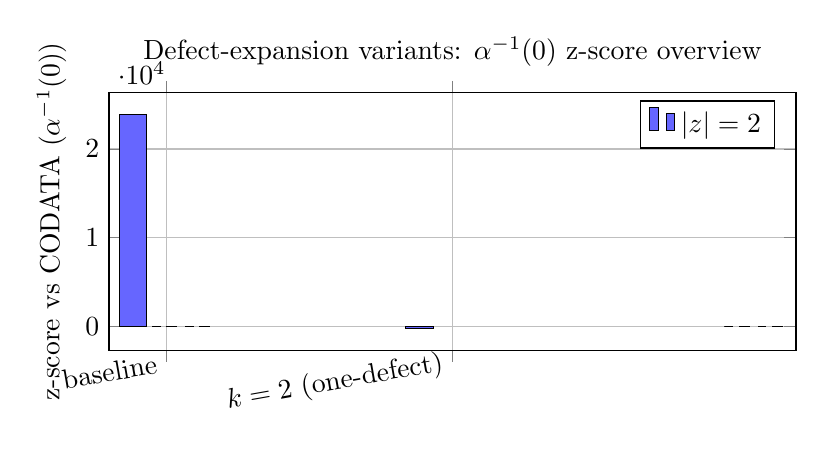
\begin{tikzpicture}
\begin{axis}[
    ybar,
    width=0.85\linewidth,
    height=0.4\linewidth,
    ylabel={z-score vs CODATA ($\alpha^{-1}(0)$)},
    title={Defect-expansion variants: $\alpha^{-1}(0)$ z-score overview},
    symbolic x coords={baseline,k2single,k2twodefectg5},
    xtick=data,
    xticklabel style={rotate=10,anchor=east},
    xticklabels={baseline,$k=2$ (one-defect),$k=2$ (two-defect, g=5)},
    grid=major,
    legend pos=north east
]
\addplot[fill=blue!60] coordinates {
    (baseline,23918.470752787038)
    (k2single,-241.68648424381988)
    (k2twodefectg5,\TFPTalphaZGOverFourNum)
};
\addplot[black, dashed] coordinates {(baseline,2) (k2twodefectg5,2)};
\addlegendentry{$|z|=2$}
\addplot[black, dashed] coordinates {(baseline,-2) (k2twodefectg5,-2)};
\end{axis}
\end{tikzpicture}
\caption{Alpha defect z-score overview. The derived two-defect ($g=5$) correction brings the CODATA discrepancy within $|z|\le 2$.}
\label{fig:alpha-defect-z}
\end{figure}

%-----------------------------------------------------------------------------
\subsection{Comparison and Scheme Policy (No Hidden Knobs)}
\label{sec:comparison-policy}
%-----------------------------------------------------------------------------

\begin{tcolorbox}[colback=yellow!3, colframe=yellow!60!black,
    title={\textbf{Primary comparison observable: $\overline{\alpha}^{(5)}(M_Z)$ ($\overline{\mathrm{MS}}$)}}, fonttitle=\bfseries\small]
\textbf{Why this matters:} Precision electroweak fits and PDG summaries use the $\overline{\mathrm{MS}}$ coupling at $M_Z$, $\overline{\alpha}^{(5)}(M_Z)$, as the comparison observable. CODATA $\alpha(0)$ is an on-shell/IR reference and is therefore treated as \emph{secondary diagnostic} once scheme and threshold bookkeeping is made explicit.

\textbf{Declared policy (suite):}
\begin{itemize}[leftmargin=1.5em, topsep=2pt, itemsep=1pt]
    \item \textbf{Primary reference:} $\overline{\alpha}^{(5)}(M_Z)^{-1} = \num{\TFPTalphaBarFiveInvMZRefNum} \pm \num{\TFPTalphaBarFiveInvMZRefSigma}$ (PDG 2024).
    \item \textbf{Secondary diagnostic:} $\alpha^{-1}(0)=\num[round-mode=places,round-precision=9]{\TFPTalphaInvCODATANum}$ (CODATA 2022).
\end{itemize}

\textbf{Result (from TFPT + declared running inputs):}
\[
\overline{\alpha}^{(5)}(M_Z)^{-1}=\num[round-mode=places,round-precision=6]{\TFPTalphaBarFiveInvMZPredNum},
\qquad
z=\num[round-mode=places,round-precision=3]{\TFPTalphaBarFiveInvMZZ}.
\]

\textbf{Reviewer-safe statement:} TFPT fixes $\alpha(0)$ via the CFE closure. The conversion to $\overline{\alpha}^{(5)}(M_Z)$ uses standard SM/QED running inputs (leptonic 1-loop, PDG hadronic vacuum polarization, and declared finite pieces), tracked by module \texttt{alpha\_precision\_audit} (Appendix~\ref{app:repro}). The inverse bridge back to $\alpha(0)$ is \emph{diagnostic only} because the CODATA uncertainty budget is not commensurate with scheme/matching systematics; the kernel/bridge split is recorded in the \texttt{alpha\_error\_ledger\_audit}.
\textbf{Evidence:} \texttt{alpha\_precision\_audit}, \texttt{alpha\_error\_ledger\_audit}.
\end{tcolorbox}

\begin{figure}[H]
\centering
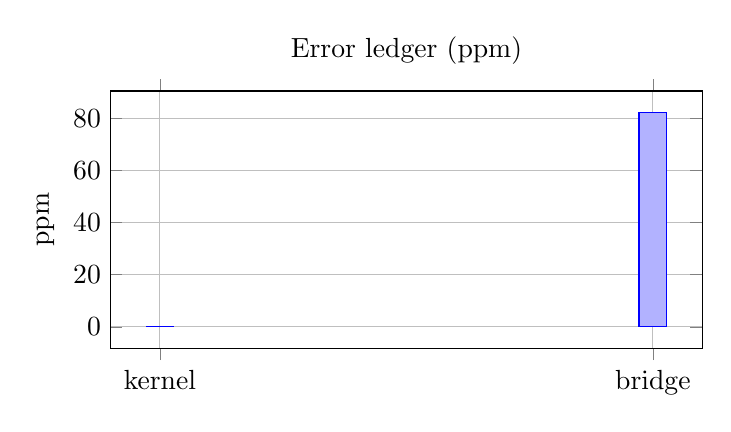
\begin{tikzpicture}
\begin{axis}[
  width=0.75\linewidth,
  height=0.40\linewidth,
  ybar,
  grid=major,
  ylabel={ppm},
  symbolic x coords={kernel,bridge},
  xtick=data,
  title={Error ledger (ppm)},
]
\addplot coordinates {(kernel,0.007178817498640309) (bridge,82.19921746062049)};
\end{axis}
\end{tikzpicture}
\caption{Kernel versus bridge uncertainty budget in ppm units (absolute magnitudes; suite ledger).}
\label{fig:error-ledger}
\end{figure}

\begin{figure}[H]
\centering
\begin{tikzpicture}
\begin{groupplot}[
    group style={group size=1 by 2, vertical sep=1.0cm},
    width=0.85\linewidth,
    height=0.32\linewidth
]
\nextgroupplot[
    xmode=log,
    xlabel={$\mu$ [GeV]},
    ylabel={$g_i$},
    title={Gauge couplings: MZ to mt (matching map)},
    title style={yshift=-0.6ex},
    grid=major,
    legend pos=north east
]
\addplot coordinates {(91.1876,0.35741704769115173) (172.76,0.3587119925553647)};
\addlegendentry{$g_Y$}
\addplot coordinates {(91.1876,0.651723832904323) (172.76,0.6483341882196387)};
\addlegendentry{$g_2$}
\addplot coordinates {(91.1876,1.2171996941475736) (172.76,1.167633324356244)};
\addlegendentry{$g_3$}

\nextgroupplot[
    xlabel={Yukawa index},
    ylabel={$y_i$ (at mt)},
    title={Yukawa proxies at mt},
    title style={yshift=-0.6ex},
    symbolic x coords={yt,yb,ytau},
    xtick=data,
    xticklabels={$y_t$,$y_b$,$y_\tau$},
    grid=major
]
\addplot[ybar, fill=blue!50] coordinates {(yt,0.9406174836767976) (yb,0.01665860318819457) (ytau,0.010214876058692106)};
\end{groupplot}
\end{tikzpicture}
\caption{MZ to mt boundary map. Explicit coupling and Yukawa boundary values under the declared MSbar policy.}
\label{fig:msbar-boundary}
\end{figure}

%=============================================================================
\section{The Unified Field Equation (UFE)}
%=============================================================================

%-----------------------------------------------------------------------------
\subsection{Quantum Vacuum Tensor Packaging}
%-----------------------------------------------------------------------------

\begin{definition}{Quantum Vacuum Tensor}{QVT}
Let
\begin{equation}
Q_{AB} := \hat{R}_{AB}(\hat{\Gamma}),
\qquad
Q^{\mathrm{TF}}_{AB} := Q_{AB} - \frac{1}{D}\hat{g}_{AB} Q^{C}{}_{C},
\qquad D:=4+n.
\end{equation}
Let $I(\alpha,L)$ denote the scalar invariant entering the coupling equation,
\begin{equation}
I(\alpha,L) := \alpha^3 - 2\cthree^3\alpha^2 - 8 \bone \cthree^6 L,
\qquad L := \ln\!\left(\frac{1}{\phiz(\alpha)}\right).
\end{equation}
Define the Quantum Vacuum Tensor
\begin{equation}
V_{AB} := Q^{\mathrm{TF}}_{AB} + \hat{g}_{AB}\, I(\alpha,L).
\end{equation}

\tcblower
\textbf{Structural equivalence principle (packaging statement).}
The vacuum law $V_{AB}=0$ splits into a scalar channel $I(\alpha,L)=0$ (CFE closure)
and a traceless ($D$-dimensional) channel $Q^{\mathrm{TF}}_{AB}=0$ (torsion vacuum equation).
This provides a compact bridge between the scalar and tensor sectors without introducing new inputs.
\end{definition}

%-----------------------------------------------------------------------------
\subsection{Torsionful Geometric Action}
%-----------------------------------------------------------------------------

\begin{definition}{UFE Action}{UFEaction}
On a manifold $M^{4+n}$ with metric $\hat{g}_{AB}$ and torsionful connection 
$\hat{\Gamma}^A_{BC}$, the action is:
\begin{equation}
    S = \int d^{4+n}x\sqrt{-\hat{g}}\left[
        \frac{1}{2\hat{\kappa}^2}\hat{R}(\hat{\Gamma}) 
        - \frac{1}{4}F_{AB}F^{AB}
        + \frac{1}{2}\hat{g}^{AB}\partial_A a\,\partial_B a 
        - V(a) 
        - \frac{\gagg}{4}\, a\, F_{AB}\tilde{F}^{AB}
    \right]
\end{equation}
Here $\hat{R}(\hat{\Gamma})$ denotes the Ricci scalar constructed from the full torsionful connection $\hat{\Gamma}$.
\end{definition}

\noindent\textbf{Minimal torsion sector.} In the parameter-free baseline we set $\mathcal{L}_{\mathrm{tors}}\equiv 0$.
All torsion dependence enters through $\hat{R}(\hat{\Gamma})$ with $\hat{\Gamma}=\Gamma(\hat{g})+K$.
The quadratic torsion treatment used for the one-loop $R^2$ completion is stated explicitly in Definition~\ref{def:R2torsion} and Appendix~\ref{app:r2}.

\noindent\textbf{Maxwell convention.} We treat the U(1) gauge potential $A$ as a one-form and define the field strength by the exterior derivative
$F := dA$, i.e.\ $F_{AB}=2\partial_{[A}A_{B]}$. This definition is independent of the torsionful affine connection $\hat{\Gamma}$; in particular, we do not use $F_{AB}=2\hat{\nabla}_{[A}A_{B]}$. Therefore U(1) gauge invariance is exact in the electromagnetic sector.

\noindent\textbf{Torsion and contorsion.} The torsion of the full connection is $T^A_{\;BC}:=2\hat{\Gamma}^A_{[BC]}$. We decompose
$\hat{\Gamma}^A_{BC}=\Gamma^A_{BC}(\hat{g})+K^A_{BC}$, where $\Gamma(\hat{g})$ is the Levi-Civita connection of $\hat{g}_{AB}$ and $K^A_{BC}$ is the contorsion tensor.

\noindent\textbf{Variational scope.} For the letter-level UFE statements we vary the metric while holding the torsionful connection fixed; no independent torsion equation of motion is required at this stage. In the core manuscript $K$ is treated as a background/auxiliary field (algebraic torsion can be integrated out); dynamical torsion is treated as an explicit extension.

\begin{theorem}{Unified Field Equations}{UFE}
Variation of the action yields the compact tensor form of the UFE. Since $\delta\hat{g}^{AB}$ is symmetric, only the symmetric part of the torsionful Ricci tensor contributes. Define
$\hat{G}_{(AB)}(\hat{\Gamma})$ by
\begin{equation*}
    \hat{G}_{(AB)}(\hat{\Gamma}) := \hat{R}_{(AB)}(\hat{\Gamma}) - \frac{1}{2}\hat{g}_{AB}\hat{R}(\hat{\Gamma}).
\end{equation*}
Then:
\begin{align}
    \hat{G}_{(AB)}(\hat{\Gamma})
        &= \hat{\kappa}^2\bigl(T^{(a)}_{AB} + T^{(\text{EM})}_{AB}\bigr)
        \label{eq:UFE}\\[0.5em]
    \nabla^{\mathrm{LC}}_A F^{AB} + \gagg(\partial_A a)\tilde{F}^{AB} &= 0
        \label{eq:maxwell}\\[0.5em]
    \nabla^{\mathrm{LC}}_A\tilde{F}^{AB} &= 0
        \label{eq:bianchi}
\end{align}
Here $\tilde{F}^{AB} := \tfrac12\,\epsilon^{ABCD}F_{CD}$ with $\epsilon^{0123}=+1$ and
metric signature $(+,-,-,-)$, and the coupling is $\gagg=-4\cthree$.
In Eqs.~\eqref{eq:maxwell}--\eqref{eq:bianchi} the covariant derivative is the Levi-Civita derivative of $\hat{g}_{AB}$ (equivalently $\nabla^{\mathrm{LC}}_A X^A=(1/\sqrt{-\hat{g}})\,\partial_A(\sqrt{-\hat{g}}\,X^A)$).
When expanding Eq.~\eqref{eq:UFE} in Levi-Civita plus contorsion variables (with $\hat{\Gamma}=\Gamma(\hat{g})+K$), all covariant derivatives are Levi-Civita.
In the torsion vacuum $(K \to 0)$, this reduces to Einstein--Hilbert gravity 
by Axiom A8.
\end{theorem}

\begin{tcolorbox}[colback=gray!5, colframe=gray!60,
title={\textbf{On-page variation for the axion--Maxwell term}}, fonttitle=\bfseries\small]
\textbf{Interaction:} $L_{\mathrm{int}}=-(\gagg/4)\,a\,F_{AB}\tilde{F}^{AB}$. \\
\textbf{Variation:} $\delta(F_{AB}\tilde{F}^{AB})=2\tilde{F}^{AB}\delta F_{AB}$ and $\delta F_{AB}=2\partial_{[A}\delta A_{B]}$. \\
\textbf{Result:} integrating by parts yields $\nabla_A F^{AB}+\gagg(\partial_A a)\tilde{F}^{AB}=0$,
matching Eq.~\eqref{eq:maxwell}.
\end{tcolorbox}

\begin{tcolorbox}[colback=gray!5, colframe=gray!60,
title={\textbf{Why the UFE uses the symmetric torsionful Einstein tensor}}, fonttitle=\bfseries\small]
Start from the torsionful Einstein--Hilbert term
\[
S_{\mathrm{EH}}=\frac{1}{2\hat{\kappa}^2}\int d^{4+n}x\,\sqrt{-\hat{g}}\;\hat{R},
\qquad
\hat{R}=\hat{g}^{AB}\hat{R}_{AB}(\hat{\Gamma}).
\]
Vary $\hat{g}^{AB}$ while holding $\hat{\Gamma}$ fixed:
\[
\delta\hat{R}=\hat{R}_{AB}\,\delta\hat{g}^{AB},
\qquad
\delta\sqrt{-\hat{g}}=-\frac12\sqrt{-\hat{g}}\;\hat{g}_{AB}\,\delta\hat{g}^{AB}.
\]
Hence $\delta S_{\mathrm{EH}}\propto\bigl(\hat{R}_{AB}-\tfrac12\hat{g}_{AB}\hat{R}\bigr)\delta\hat{g}^{AB}$.
Since $\delta\hat{g}^{AB}$ is symmetric, only the $(AB)$ part contributes, so the unambiguous vacuum equation is
\[
\hat{G}_{(AB)}(\hat{\Gamma})\equiv \hat{R}_{(AB)}(\hat{\Gamma})-\frac12\hat{g}_{AB}\hat{R}(\hat{\Gamma})=0.
\]
\end{tcolorbox}

\begin{tcolorbox}[colback=gray!5, colframe=gray!60,
title={\textbf{Notation: Ricci tensor under }\(\hat{\Gamma}=\Gamma(\hat{g})+K\)}, fonttitle=\bfseries\small]
We use $\nabla$ for the Levi-Civita derivative of $\hat{g}_{AB}$ in this decomposition.
Define the contracted rank-two tensors
\[
(\nabla K)_{BD}:=\nabla_A K^A{}_{DB}-\nabla_D K^A{}_{AB},
\qquad
(K^2)_{BD}:=K^A{}_{AE}K^E{}_{DB}-K^A{}_{DE}K^E{}_{AB}.
\]
With these conventions the identity is literal:
\[
\hat{R}_{BD}=R_{BD}+(\nabla K)_{BD}+(K^2)_{BD}.
\]
\end{tcolorbox}

\begin{tcolorbox}[colback=blue!3, colframe=blue!40,
    title={\textbf{Lemma (Torsion-Induced Bounce Term)}}, fonttitle=\bfseries\small]
In Einstein--Cartan-type setups where torsion is algebraic, integrating out the
axial torsion produces an effective spin--spin interaction
$(\bar{\psi}\gamma_5\gamma_\mu\psi)^2$. In a homogeneous cosmological background this term
scales as $a^{-6}$ and contributes a repulsive component at small scale factor,
allowing a non-singular bounce. This provides the minimal bridge from the UFE to
bounce scenarios used in Sec.~\ref{sec:bounce}.
\end{tcolorbox}

%-----------------------------------------------------------------------------
\subsection{Present-Day Torsion Regimes and Local Tests}
\label{sec:torsion-regimes}
%-----------------------------------------------------------------------------

TFPT distinguishes between \emph{cosmological torsion} (which may be active in the early universe and drive a bounce) and \emph{local vacuum torsion} (which is constrained by laboratory and astrophysical bounds on Lorentz violation).
To avoid hidden assumptions, we treat ``torsion today'' as an explicit regime choice rather than a vague qualitative statement.

\begin{tcolorbox}[colback=yellow!3, colframe=yellow!60!black,
    title={\textbf{Regime declaration (baseline vs.\ falsifiable alternatives)}}, fonttitle=\bfseries\small]
\textbf{Baseline (suite):} local vacuum torsion today vanishes,
\[
S_\mu(\text{today})=0,
\]
so local bounds are automatically satisfied and only cosmological torsion dynamics remain relevant for early-universe completions (bounce, condensates).

\textbf{Falsifiable alternatives:} if a TFPT completion predicts a nonzero local $S_\mu$, it must lie below the component-wise bounds and should be stated as a concrete regime proposal (the suite provides an exportable JSON ``regime designer'' to make such proposals explicit).
\end{tcolorbox}

\TFPTTorsionBoundsTable

\begin{figure}[H]
\centering
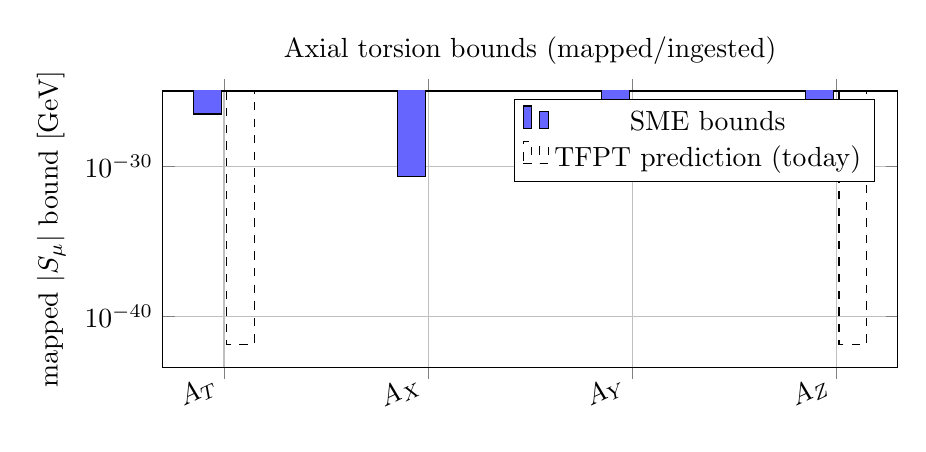
\begin{tikzpicture}
\begin{axis}[
    ybar,
    ymode=log,
    width=0.9\linewidth,
    height=0.42\linewidth,
    ylabel={mapped $|S_\mu|$ bound [GeV]},
    title={Axial torsion bounds (mapped/ingested)},
    symbolic x coords={AT,AX,AY,AZ},
    xtick=data,
    xticklabel style={rotate=25,anchor=east},
    xticklabels={$A_T$,$A_X$,$A_Y$,$A_Z$},
    grid=major,
    legend pos=north east
]
\addplot[fill=blue!60] coordinates {(AT,2.9e-27) (AX,2.1e-31) (AY,2.5e-31) (AZ,1.0e-29)};
\addlegendentry{SME bounds}
\addplot[black, dashed] coordinates {(AT,1.436869415091482e-42) (AZ,1.436869415091482e-42)};
\addlegendentry{TFPT prediction (today)}
\end{axis}
\end{tikzpicture}
\caption{Axial torsion bounds (mapped). SME coefficients $A_\mu$ (x-axis labels) translated to $|S_\mu|$ with explicit mapping; the TFPT baseline $S_\mu(\text{today})=0$ is shown at a small floor value for the log scale.}
\label{fig:torsion-bounds}
\end{figure}

\begin{tcolorbox}[colback=gray!5, colframe=gray!60,
    title={\textbf{Two concrete torsion test benchmarks (suite; regime designer)}}, fonttitle=\bfseries\small]
The suite includes an explicit ``regime designer'' that translates spin-polarized media into a toy torsion estimate and compares it to vetted component-wise bounds (module \texttt{ux\_torsion\_regime\_designer}). 
The intent is not to claim a derived microscopic coupling here, but to make \emph{testability regimes} concrete.
\end{tcolorbox}

\begin{table}[H]
\centering
\begin{tabular}{@{}llll@{}}
\toprule
\textbf{Benchmark} & \textbf{Coupling scale} & \textbf{Density} & \textbf{$|S_\mu|$ for $c_{\rm spin}=1$ [GeV]} \\
\midrule
Electron gas (lab) & $M_{\rm Pl}^{-1}$ & $n\sim 10^{23}\,\mathrm{cm^{-3}}$ & $\sim \num{3.24e-56}$ \\
Nuclear matter core & TFPT $M^{-1}$ & $n\sim 0.16\,\mathrm{fm^{-3}}$ & $\sim \num{3.28e-31}$ \\
\bottomrule
\end{tabular}
\caption{Order-of-magnitude torsion benchmarks from the suite module \texttt{ux\_torsion\_regime\_designer}. In the lab benchmark, the signal is hopelessly small under Planck coupling; in dense matter under TFPT-$M$ coupling, the estimate approaches current bounds (depending on the effective $c_{\rm spin}$).}
\end{table}

\begin{figure}[H]
\centering
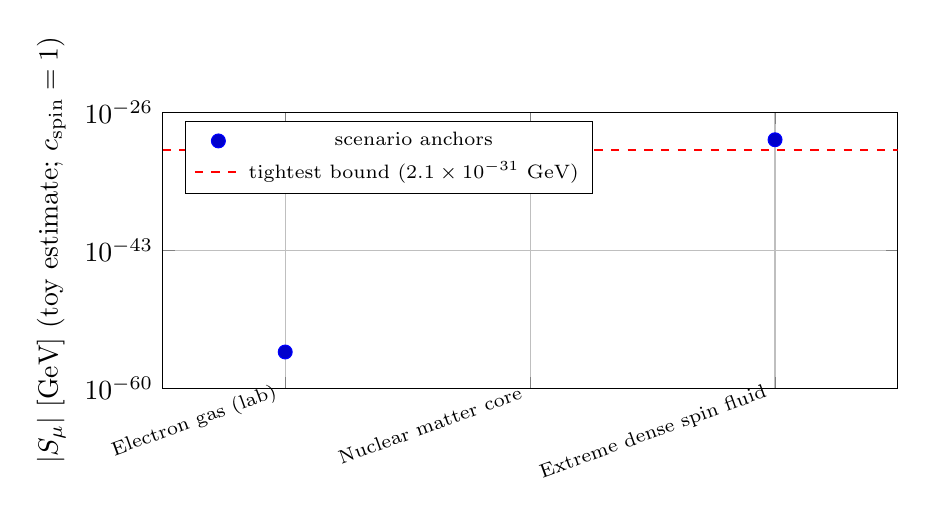
\begin{tikzpicture}
\begin{axis}[
    width=0.9\linewidth,
    height=0.42\linewidth,
    ymode=log,
    ymin=1e-60, ymax=1e-26,
    xmin=0.5, xmax=3.5,
    xtick={1,2,3},
    xticklabels={Electron gas (lab), Nuclear matter core, Extreme dense spin fluid},
    x tick label style={rotate=20, anchor=east, font=\scriptsize},
    ylabel={$|S_\mu|$ [GeV] (toy estimate; $c_{\rm spin}=1$)},
    grid=both,
    legend style={font=\scriptsize},
    legend pos=north west,
]
\addplot+[only marks, mark=*, mark size=2.5pt] coordinates {
    (1,3.2396753580225e-56)
    (2,3.2832238430084956e-31)
    (3,4.104029803760619e-30)
};
\addlegendentry{scenario anchors}

\addplot[red, dashed, thick] coordinates {(0.5,2.1e-31) (3.5,2.1e-31)};
\addlegendentry{tightest bound ($2.1\times10^{-31}$ GeV)}
\end{axis}
\end{tikzpicture}
\caption{Suite regime scan (\texttt{ux\_torsion\_regime\_designer}): torsion estimates and bound-saturation targets across illustrative spin-medium scenarios.}
\end{figure}

%-----------------------------------------------------------------------------
